\section{Method}
\label{sec:method}

\subsection{Overview}
\label{sec:method_overview}

CoM3D-ACE is designed around one principle: ambiguous UAV detections should be
converted into explicit evidence before they are fused, completed, or reasoned
over. Given synchronized UAV observations
$\mathcal{I}=\{(I_i, K_i, T_i, t_i)\}_{i=1}^{N}$ with image $I_i$, camera
intrinsics $K_i$, camera pose $T_i$, and timestamp $t_i$, the system first
extracts 2D object evidence with SAFR-YOLO. Each detection is then represented
as an EvidenceToken and inserted into a cross-view 3D evidence graph. The graph
routes confident hypotheses to a verified object state and routes ambiguous
hypotheses to 3D completion, re-observation, and AeroGraph reasoning.

\begin{figure*}[t]
\centering
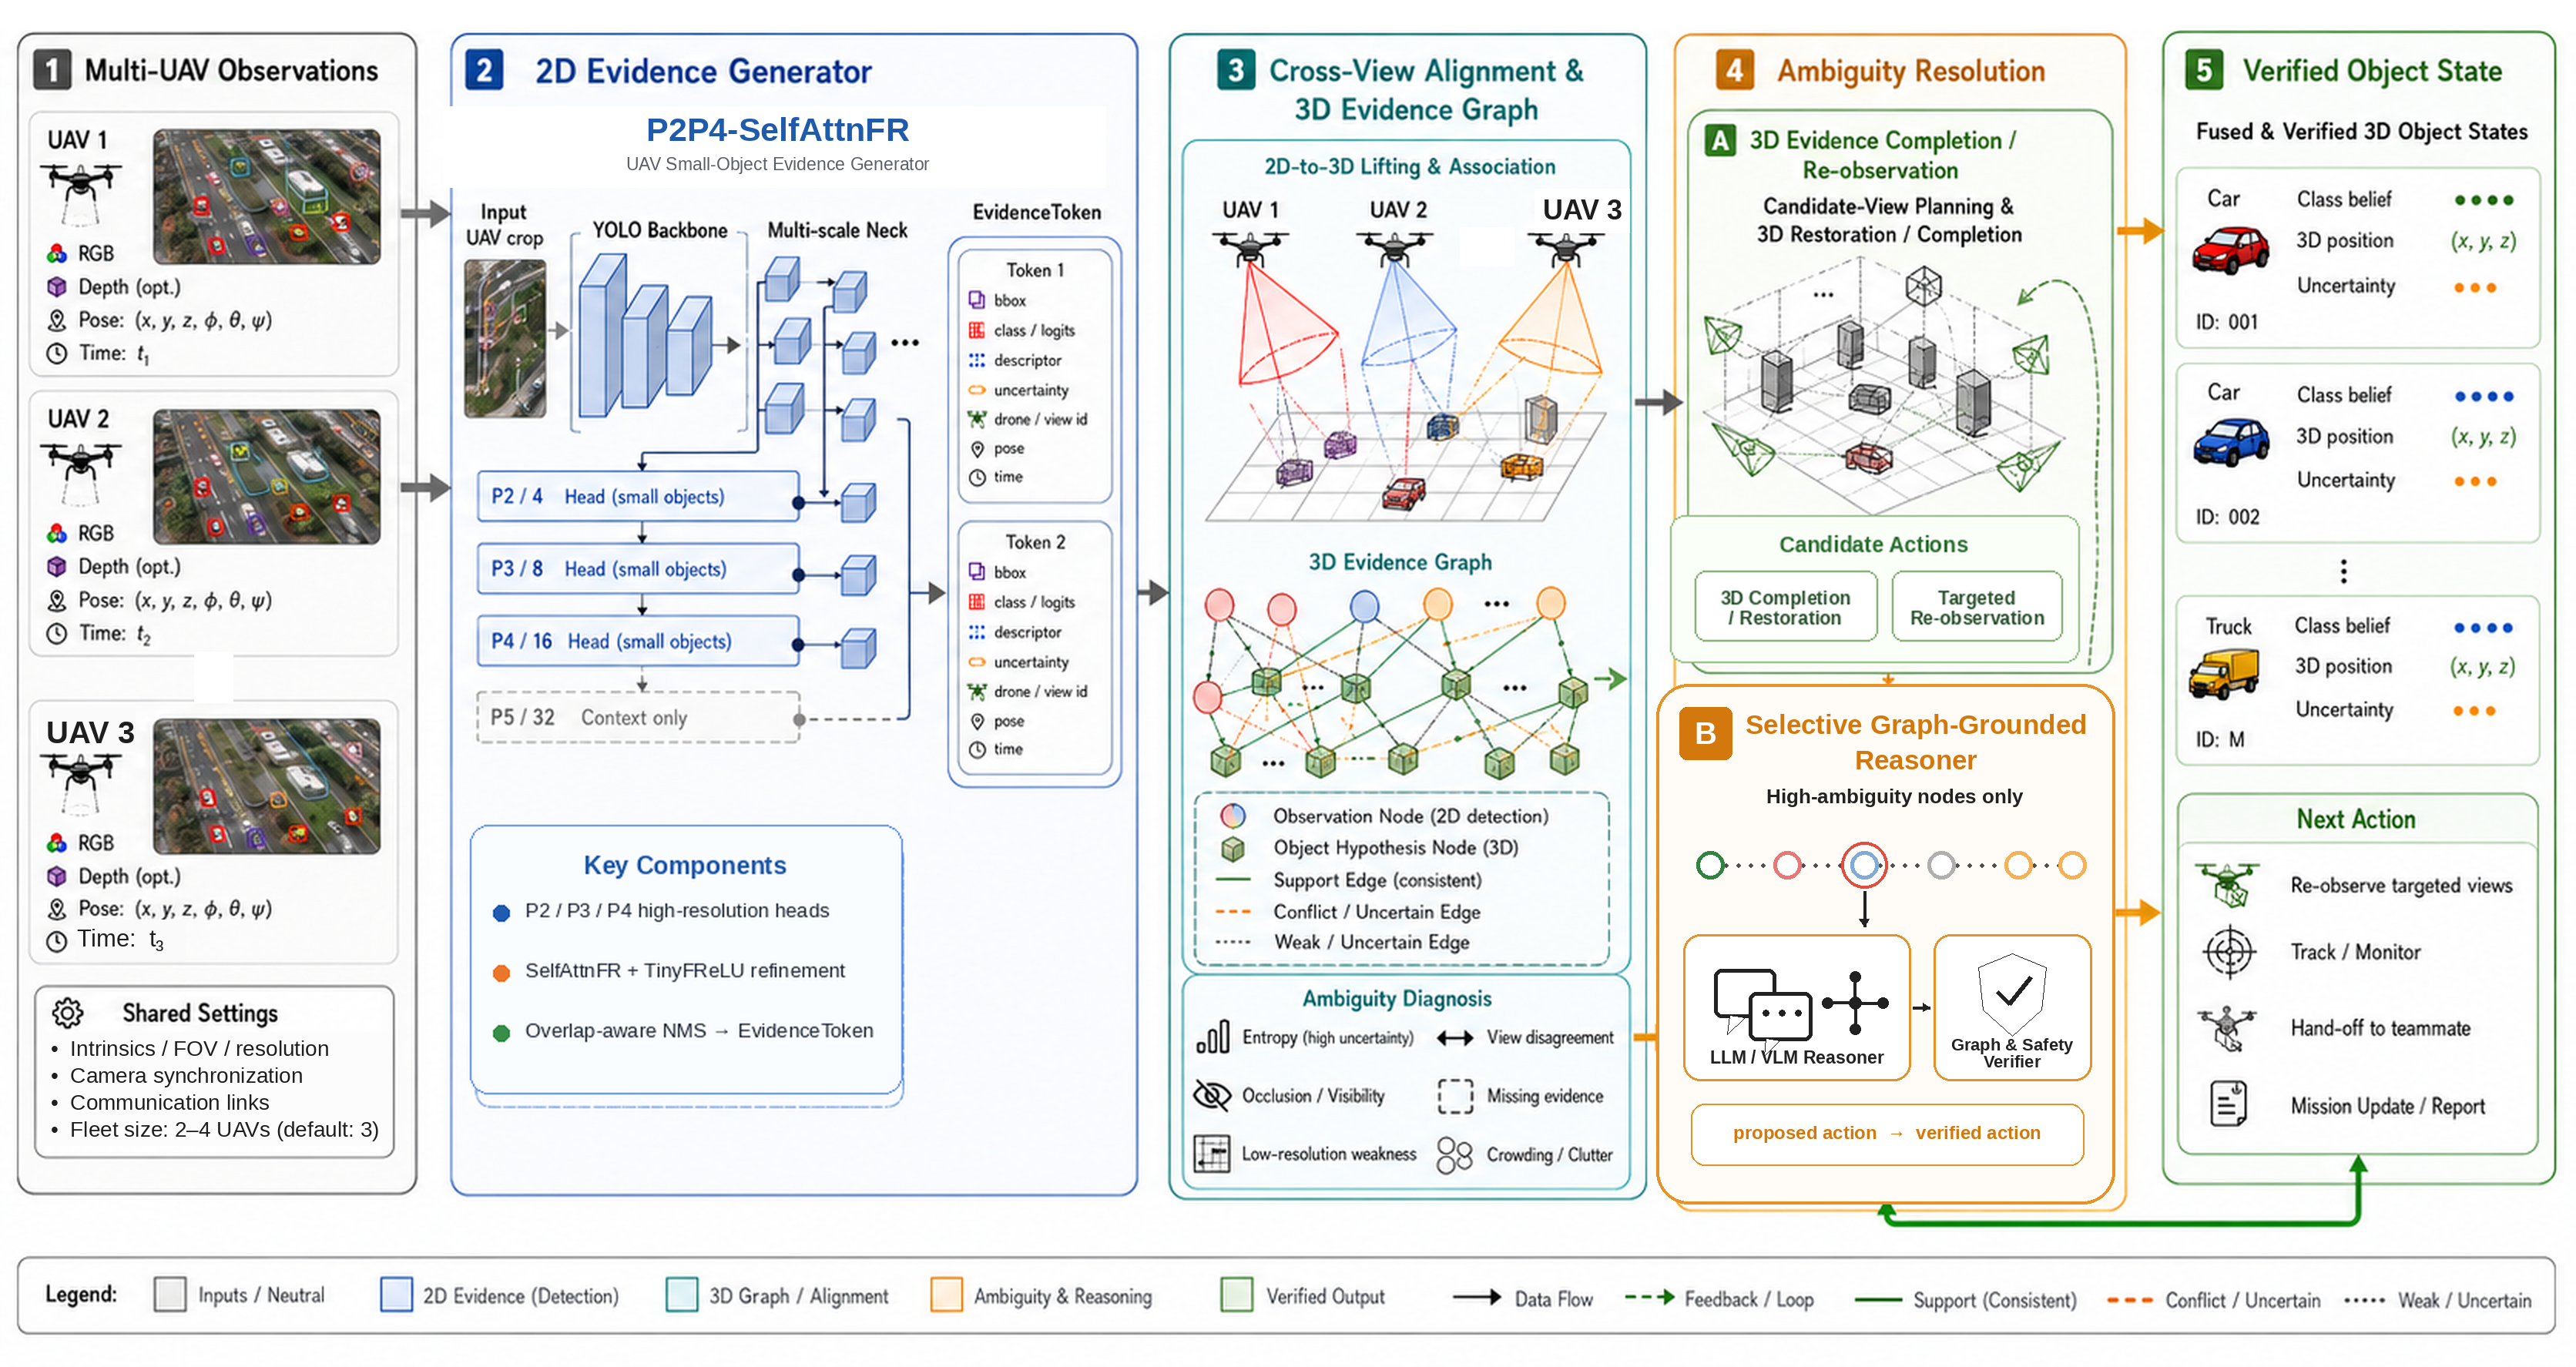
\includegraphics[width=0.98\textwidth]{figures/fig01_com3d_ace_overall_framework.png}
\caption{CoM3D-ACE overview. Multi-UAV observations are converted by SAFR-YOLO
into EvidenceTokens, associated into a 3D evidence graph, and routed to 3D
completion, targeted re-observation, and the graph-grounded AeroGraph Reasoner
only when ambiguity remains high.}
\label{fig:com3d_ace_overview}
\end{figure*}

\subsection{SAFR-YOLO 2D Evidence Generator}
\label{sec:method_safr_yolo}

SAFR-YOLO follows a YOLO-family backbone--neck--head structure but changes the
small-object prediction path. The P2/P3/P4 feature maps are used as the primary
detection heads, while the P5/32 branch is retained as semantic context rather
than a final small-object prediction head. This matches the observation that
very coarse feature maps are weak for tiny aerial targets.

The selected implementation, P2P4-SelfAttnFR, adds SelfAttnFR refinement before
the detection heads. SelfAttnFR has two lightweight paths. The first path pools
the spatial feature map into a small set of tokens and applies self-attention to
capture adjacent-object context at low cost. The second path applies local
refinement and TinyFReLU to preserve high-frequency edge and texture cues. The
two paths are fused with a $1\times1$ projection before detection.

\begin{figure*}[t]
\centering
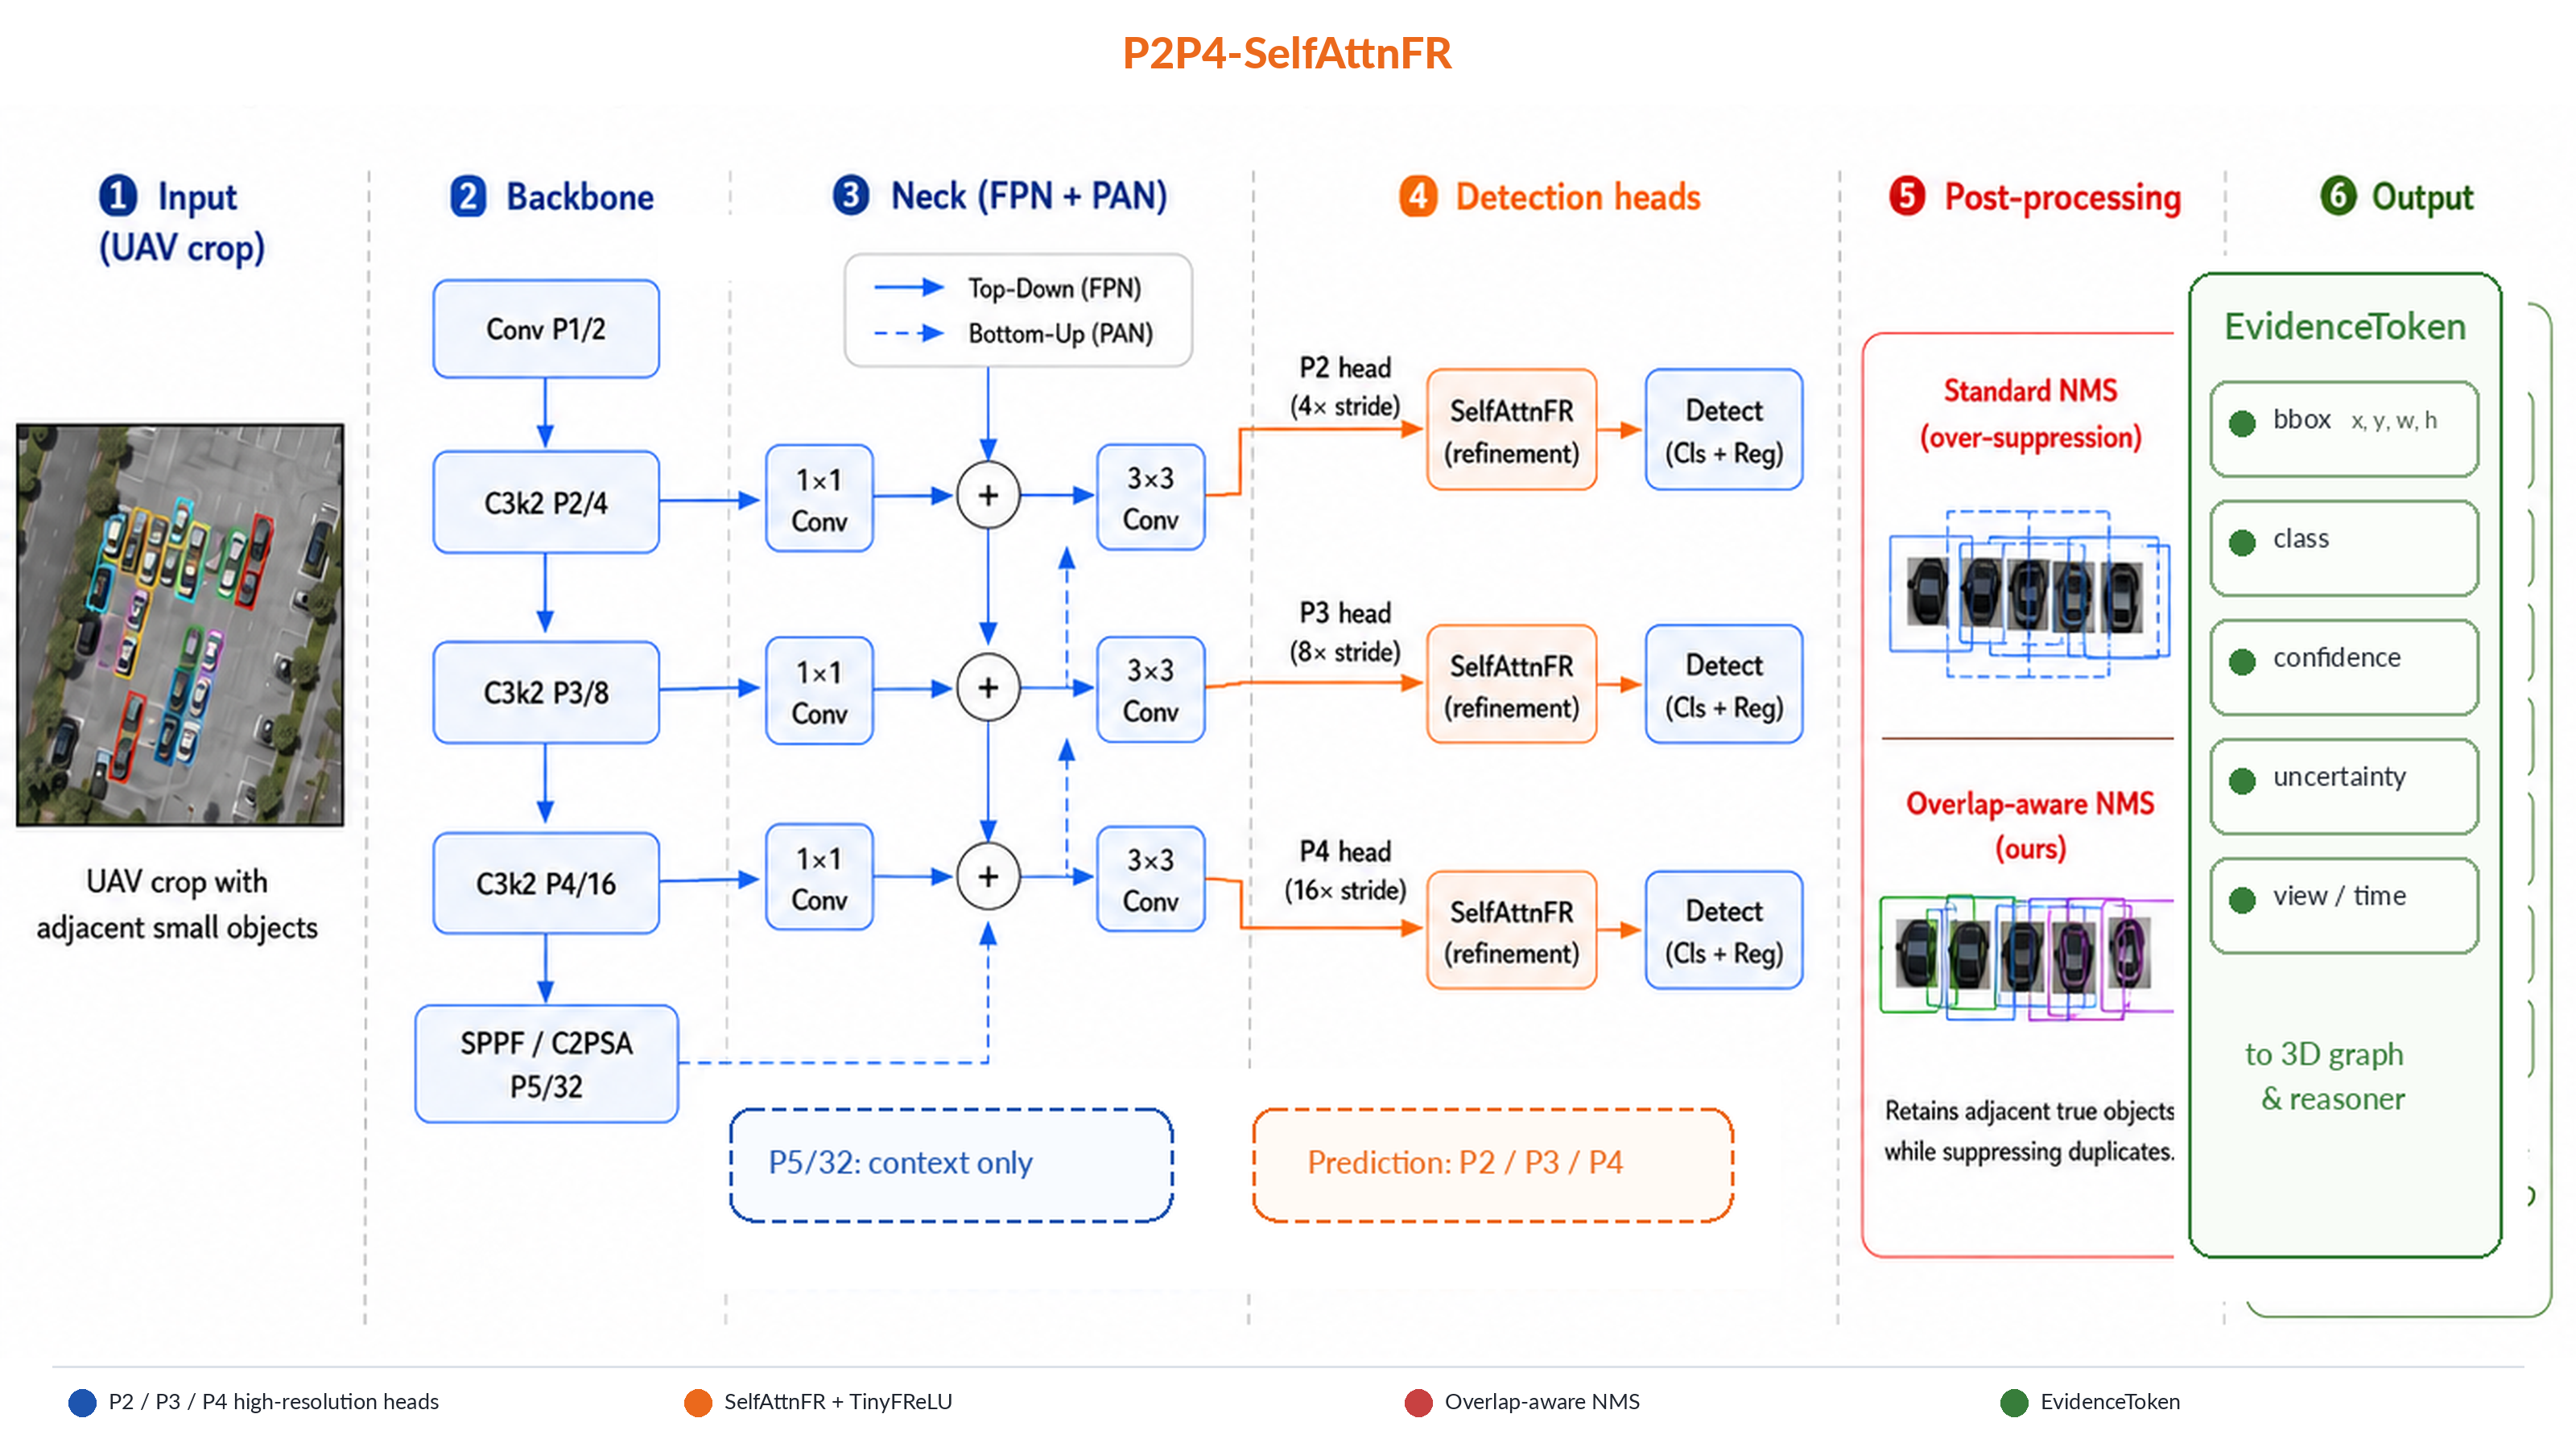
\includegraphics[width=0.98\textwidth]{figures/fig02_p2p4_safr_yolo.png}
\caption{SAFR-YOLO detector structure. P2/P3/P4 heads provide high-resolution
small-object predictions, SelfAttnFR refines adjacent-object context and local
detail, and overlap-aware post-processing exports EvidenceTokens for downstream
3D reasoning.}
\label{fig:safr_yolo}
\end{figure*}

For an input feature $F\in\mathbb{R}^{H\times W\times C}$, TinyFReLU uses a
depthwise spatial condition and a high-frequency residual:
\begin{equation}
h(x)=x-\mathrm{AvgPool}_{3\times3}(x),
\end{equation}
\begin{equation}
c(x)=\mathrm{BN}(\mathrm{DWConv}_{3\times3}(x))+\tanh(\gamma)h(x),
\end{equation}
\begin{equation}
y=\max(x,c(x)).
\end{equation}
This keeps the activation close to a lightweight FReLU-style gate
\cite{ma2020frelu} while adding an explicit residual cue for weak tiny-object
boundaries. The overlap-aware post-processing used in SAFR-YOLO is evaluated
against standard NMS and Soft-NMS-style alternatives \cite{bodla2017softnms}
to avoid suppressing adjacent tiny objects solely because their boxes overlap.

\subsection{EvidenceToken Representation}
\label{sec:method_evidence_token}

Each detector output is converted into an EvidenceToken:
\begin{equation}
\tau = (b, p, s, u, f, v, T, t),
\end{equation}
where $b=(x,y,w,h)$ is the bounding box, $p$ is the class-logit vector, $s$ is
the confidence score, $u$ is an uncertainty descriptor, $f$ is an optional crop
or feature descriptor, $v$ is the UAV/view identifier, $T$ is the camera pose,
and $t$ is the timestamp. This representation keeps the detector output
compatible with ordinary 2D evaluation while exposing the fields required for
cross-view association.

\subsection{Cross-View 3D Evidence Graph}
\label{sec:method_evidence_graph}

The EvidenceTokens are associated into a graph
$\mathcal{G}=(\mathcal{V},\mathcal{E})$. Observation nodes represent 2D tokens,
and object-hypothesis nodes represent candidate 3D object states. Edges encode
support, conflict, or missing evidence. A token supports a hypothesis when its
view ray, class belief, and descriptor are consistent with the hypothesis. It
creates conflict evidence when the class belief or projected geometry disagrees,
and missing-evidence edges mark views where an object should be observable but
was not confidently detected.

We compute an ambiguity score for each hypothesis:
\begin{equation}
A(o)=\lambda_H H(p_o)+\lambda_D D_o+\lambda_M M_o+\lambda_C C_o,
\end{equation}
where $H(p_o)$ is class-belief entropy, $D_o$ measures view disagreement,
$M_o$ counts missing-view evidence, and $C_o$ summarizes crowding or overlap
conflicts. Low-ambiguity hypotheses can be finalized directly. High-ambiguity
hypotheses are routed to 3D completion, targeted re-observation, or AeroGraph
Reasoner validation.

\subsection{MarineCity 3D Evidence Completion And AeroGraph Reasoner}
\label{sec:method_3d_reasoner}

For MarineCity experiments, the system exports real-Cesium RGB/depth/pose
captures and a NeRF-style transforms package. Neural-3D runners are used to
test whether the capture package can support held-out viewpoint reconstruction
and completion. The resulting 3D evidence is not treated as a replacement for
2D detection; it is used as additional context for ambiguous object hypotheses.

\begin{figure*}[t]
\centering
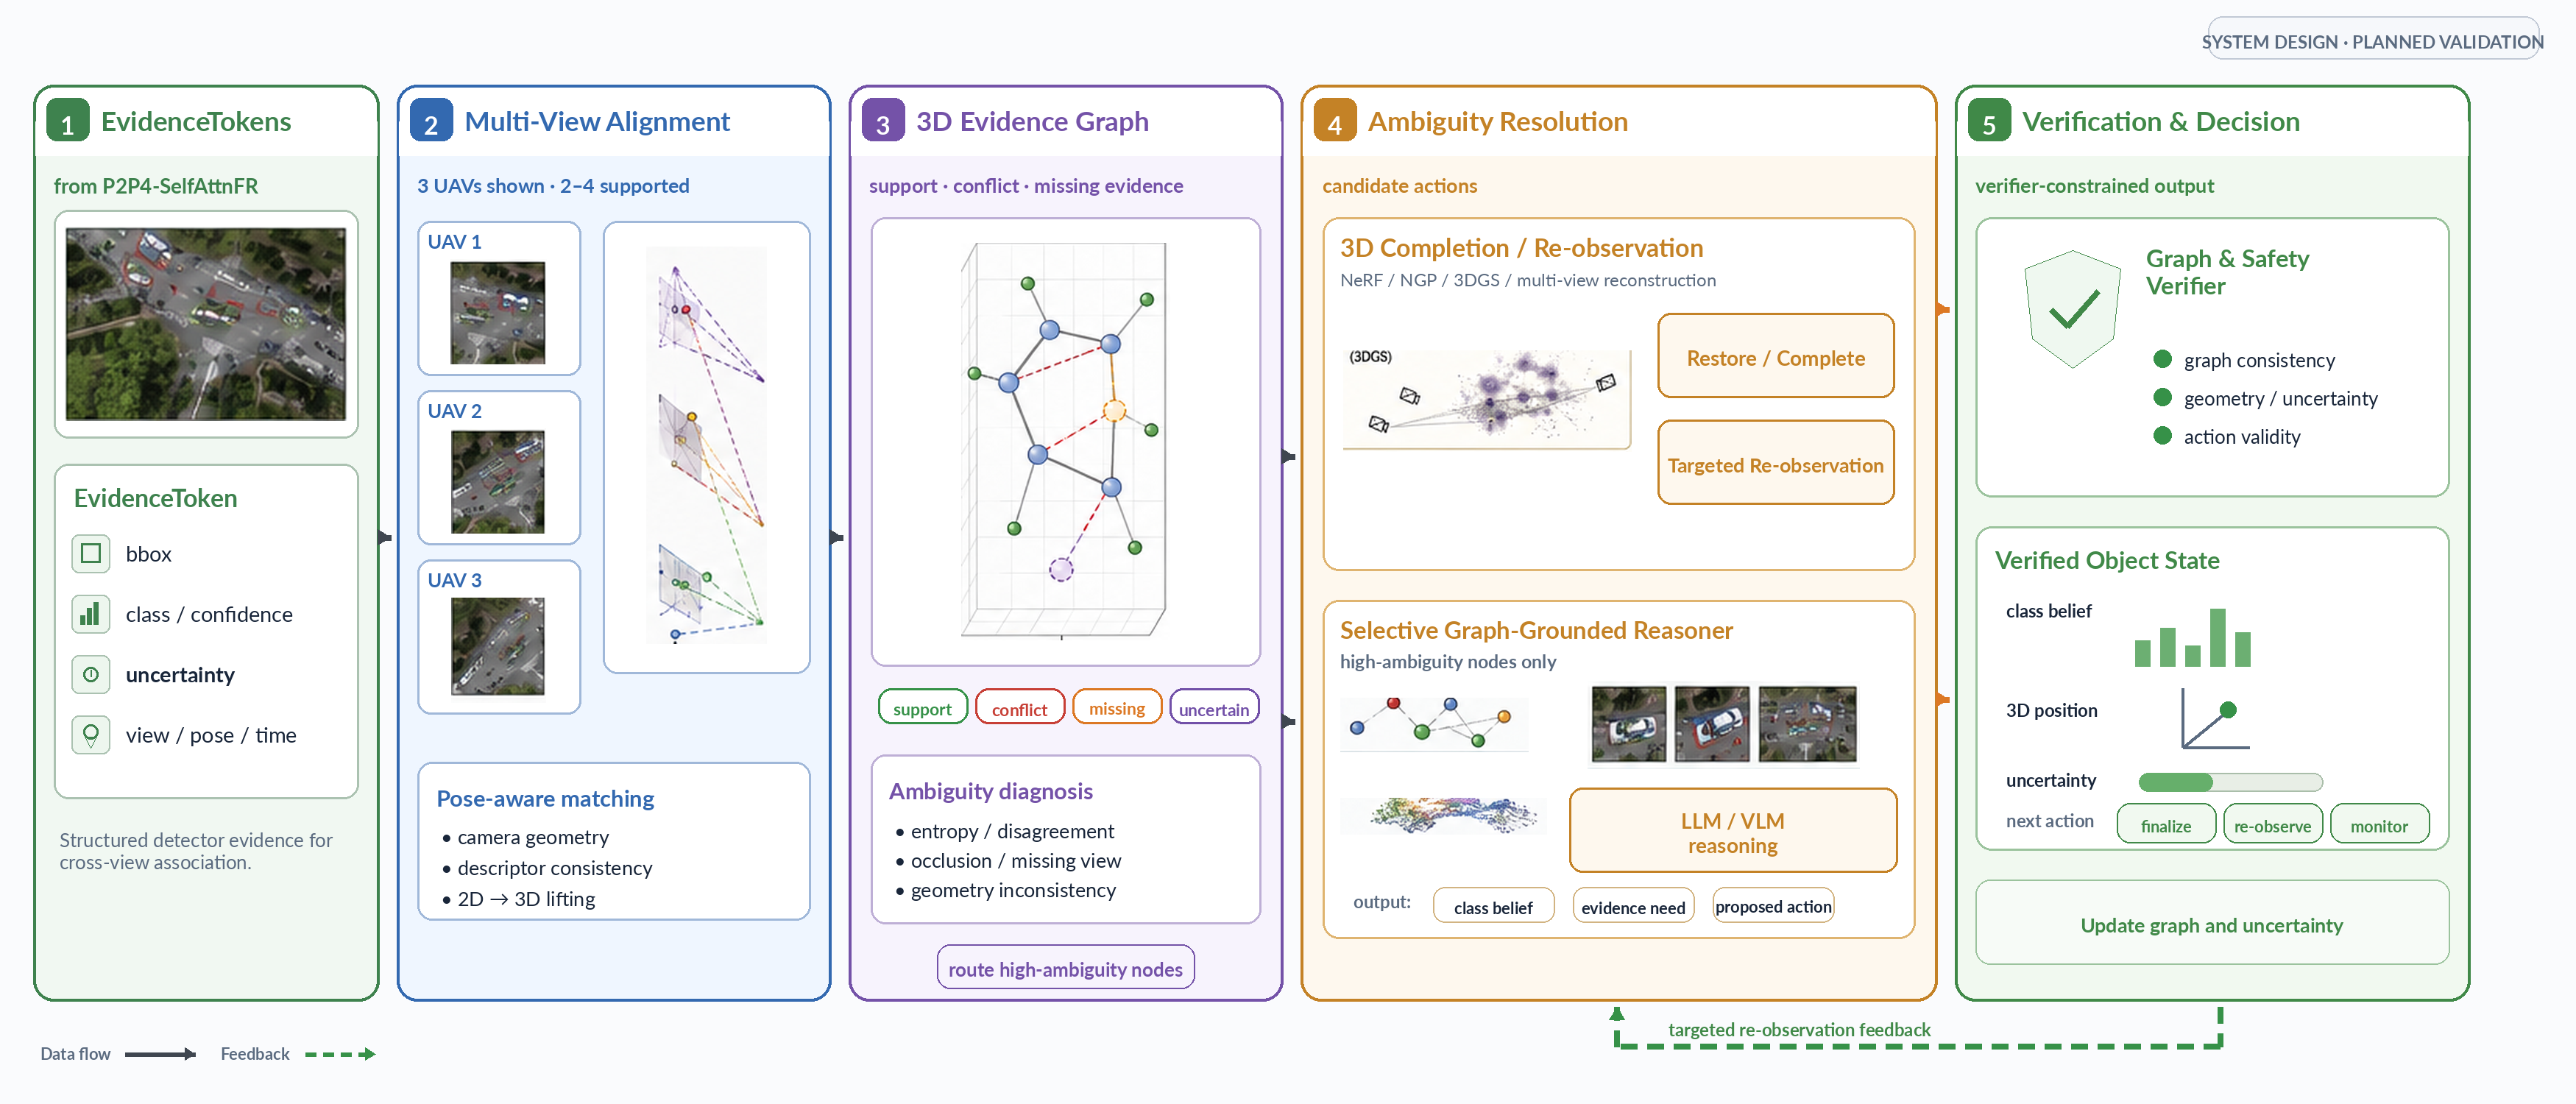
\includegraphics[width=0.98\textwidth]{figures/fig03_3d_evidence_reasoner.png}
\caption{3D evidence completion and AeroGraph Reasoner interface. The current
paper reports real-Cesium system/protocol validation and neural-3D
runner-family smoke metrics; external-provider reasoning results are kept as a
separate validation slot.}
\label{fig:marinecity_3d_reasoner}
\end{figure*}

The AeroGraph Reasoner receives a compact graph-grounded package containing the
high-ambiguity subgraph, supporting and conflicting crops, a geometry summary,
and allowed actions. It returns a structured decision containing class belief,
confidence, evidence needs, and a proposed action. A graph-and-safety verifier
checks whether the action is consistent with the evidence graph and physically
plausible before it is accepted.
